\chapter{Plots}\label{ch:plots}

\texttt{nwsbmplot} draws pictures of the last fit. The network and the membership probabilities must still be in memory, except for \opt{type(icl)}, which works from the stored table.

\section{Syntax and options}
\begin{lstlisting}
nwsbmplot [, type(matrix|expected|membership|blocks|icl) options]
\end{lstlisting}
\begin{longtable}{@{}p{0.30\textwidth}p{0.66\textwidth}@{}}
\toprule
Option & Meaning\\
\midrule
\endhead
\opt{type(type)} & \opt{matrix} (default, alias \opt{data}), \opt{expected}, \opt{membership}, \opt{blocks} (alias \opt{meso}) or \opt{icl}\\
\opt{shade} & matrix: shade the block rectangles by their connectivity (four levels, relative to the largest entry of \texttt{e(pi)})\\
\opt{nolines} & matrix, expected, membership: no lines between the blocks\\
\opt{missing} & matrix: show pairs with a missing tie\\
\opt{nolabels} & matrix, expected: no block numbers on the axes\\
\opt{blocklabels(list)} & names of the blocks (mode 1 first, then mode 2) for the axes, the legend of membership and the nodes of blocks\\
\opt{actorlabels(varname)} & matrix, expected, membership: names of the actors (string variable, or numeric with value labels) on the axes or under the bars; up to 40 actors, otherwise ignored with a note\\
\opt{linecolor(color)} & matrix, expected: colour of the lines between the blocks; default \texttt{gs8}\\
\opt{nolegend} & icl, membership: no legend box\\
\opt{sort} & matrix, expected: within a block order the actors by decreasing certainty\\
\opt{colors(list)} & colours of the blocks (blocks, membership, icl): \texttt{default}, \texttt{gray} or a list of Stata colour names\\
\opt{title(text)} & title of the graph; \texttt{title("")} draws no title\\
\opt{name(name)} & name of the graph in memory\\
\opt{saving(filename)} & save the graph as a \texttt{.gph} file\\
\opt{export(filename)} & export the graph with \texttt{graph export} (\texttt{.png}, \texttt{.pdf}, \texttt{.eps}, \dots{} by the extension; an existing file is replaced)\\
\emph{twoway\_options} & other options of \texttt{twoway}, such as \texttt{xtitle()}, \texttt{xsize()} or \texttt{subtitle()}; they come last and override the defaults\\
\bottomrule
\end{longtable}
Titles, subtitles, axis titles and legend titles are black by default. The figures below were made with the scheme \texttt{s1network} of the core and, where a plot colours the blocks, with \opt{colors(gray)}.

\section{The plot types}
\paragraph{Blocked adjacency matrix.} \opt{type(matrix)} draws every tie as a point in the adjacency matrix with the actors ordered by their most probable block, so that the block structure shows as dense and sparse rectangles; valued ties are darker for larger values. Figure~\ref{fig:matrix} shows the two-block fit of the karate club (command in the caption); the rows and columns of the small, dense block are crowded with ties.
\begin{figure}[htbp]\centering
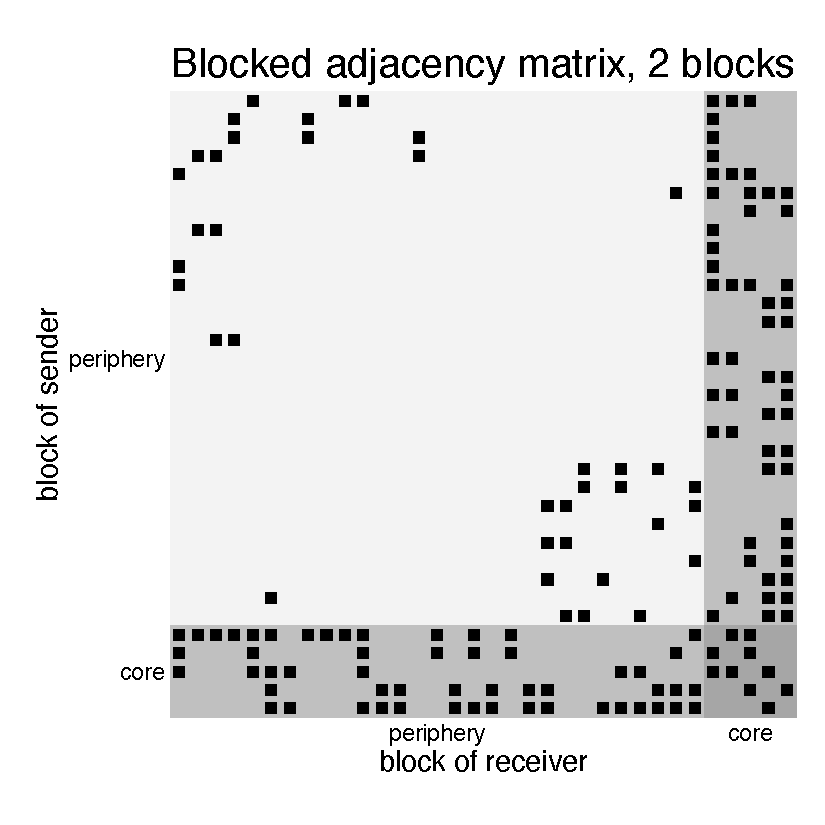
\includegraphics[width=0.62\textwidth]{fig/fig_matrix.pdf}
\caption{\texttt{nwsbmplot, type(matrix) shade blocklabels(periphery core)} after the two-block fit of the karate club.}\label{fig:matrix}
\end{figure}

\paragraph{ICL against the number of blocks.} \opt{type(icl)} draws the ICL of every fitted number of blocks and marks the selected one with a diamond (Figure~\ref{fig:icl}). With \opt{icl(exact)} it draws the exact ICL and, on a second axis, the ICL of \blockmodels{} (Figure~\ref{fig:iclexact}). For a two-mode network there is one line per number of blocks of mode~2 over the number of blocks of mode~1 (Figure~\ref{fig:davisicl}). It needs at least two fitted numbers of blocks.
\begin{figure}[htbp]\centering
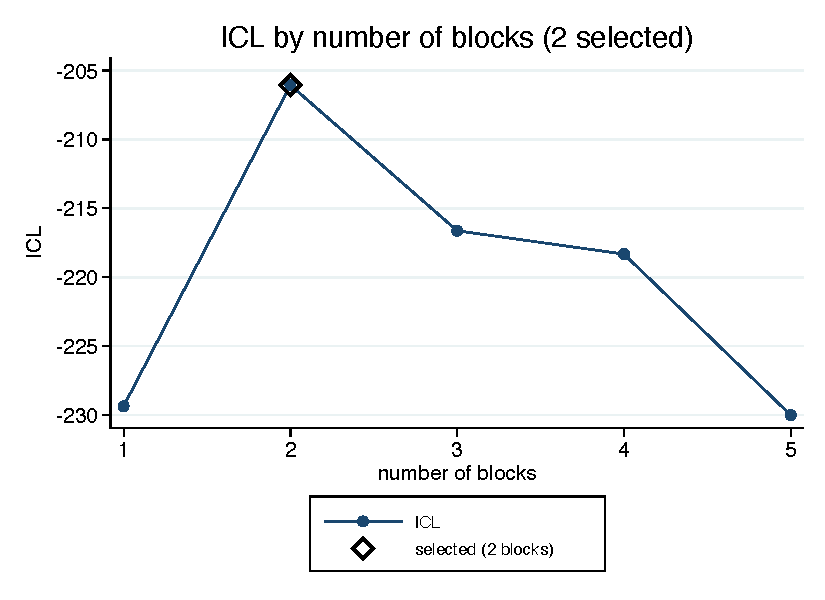
\includegraphics[width=0.7\textwidth]{fig/fig_icl.pdf}
\caption{\texttt{nwsbmplot, type(icl)}, karate club, one to five blocks.}\label{fig:icl}
\end{figure}
\begin{figure}[htbp]\centering
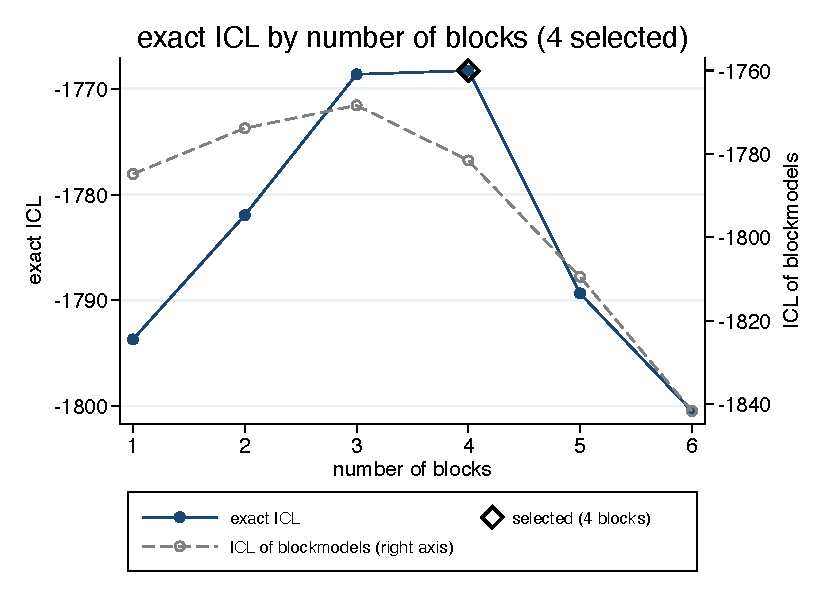
\includegraphics[width=0.7\textwidth]{fig/fig_iclexact.pdf}
\caption{\texttt{nwsbmplot, type(icl)} after a fit of the law firm's friendship network with \texttt{icl(exact)}: the exact ICL (left axis) and the ICL of \texttt{blockmodels} (right axis).}\label{fig:iclexact}
\end{figure}
\begin{figure}[htbp]\centering
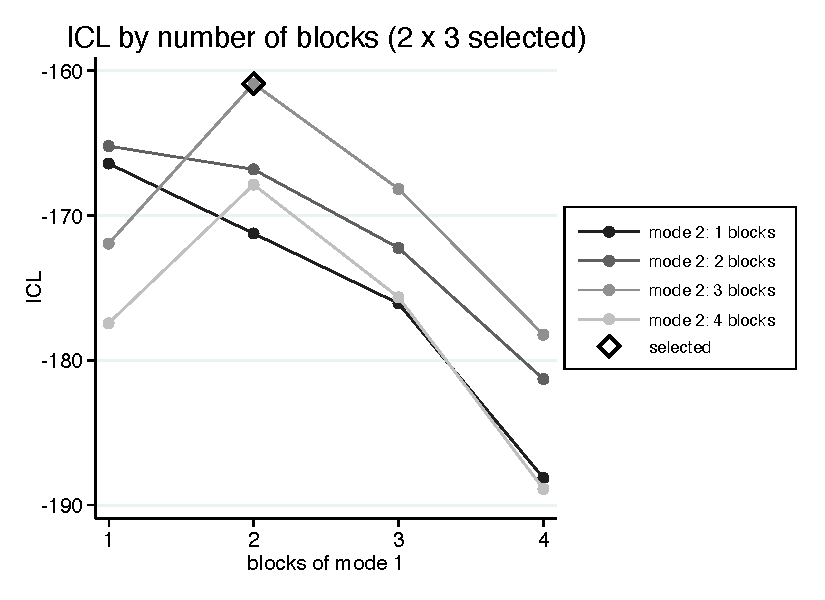
\includegraphics[width=0.62\textwidth]{fig/fig_davisicl.pdf}
\caption{\texttt{nwsbmplot, type(icl) colors(gray)} after the two-mode fit of the Southern women with \texttt{maxblocks(4 4)}.}\label{fig:davisicl}
\end{figure}

\paragraph{Expected ties.} \opt{type(expected)} draws the posterior expected value of every tie, $E=T_1\,\pi\,T_2'$, where $T_1$ and $T_2$ hold the membership probabilities of the actors, with the actors ordered as in the matrix plot and eight grey levels spanning the range of the values (the range is in the subtitle). It shows the block part of the model only: the degree parameters and the covariate terms are not included. In a one-mode network the diagonal is left out; at most 2.5 million cells are drawn. Figure~\ref{fig:expected} shows it for the friendship network of the law firm, with \opt{sort} (within a block, actors by decreasing certainty).
\begin{figure}[htbp]\centering
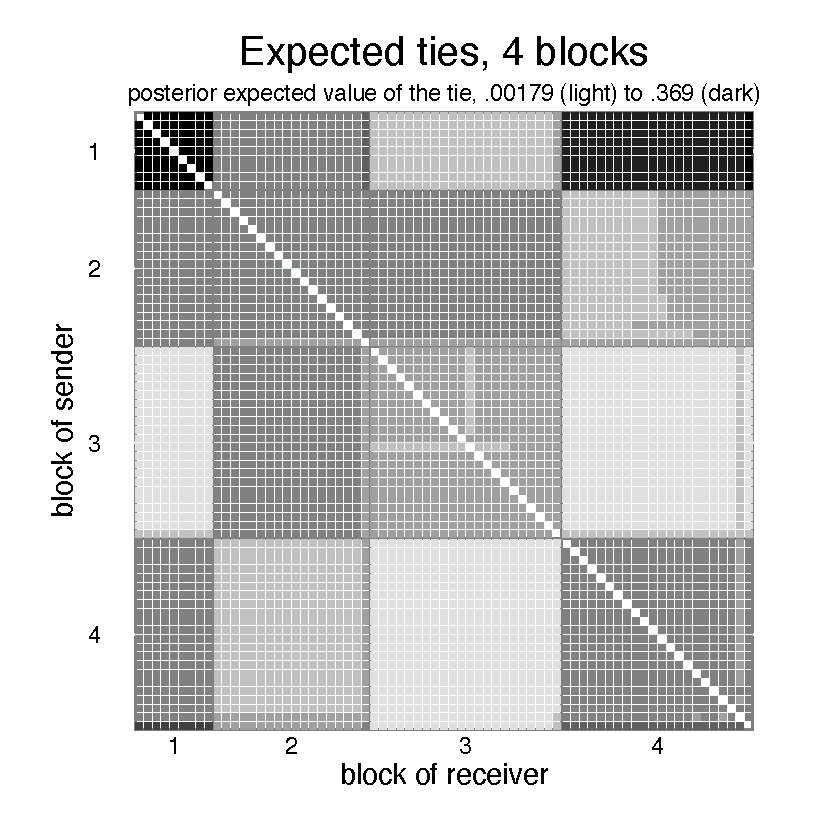
\includegraphics[width=0.7\textwidth]{fig/fig_expected.pdf}
\caption{\texttt{nwsbmplot, type(expected) sort} after the four-block fit of the law firm's friendship network (exact ICL).}\label{fig:expected}
\end{figure}

\paragraph{Memberships.} \opt{type(membership)} draws the membership probabilities as stacked bars, one colour per block, the actors ordered by their most probable block and within it by decreasing certainty; blocks that are not clear-cut show as mixed bars. For a two-mode network there is one panel per mode. In Figure~\ref{fig:member} nearly all bars of the karate club have one colour: the memberships are sharp.
\begin{figure}[htbp]\centering
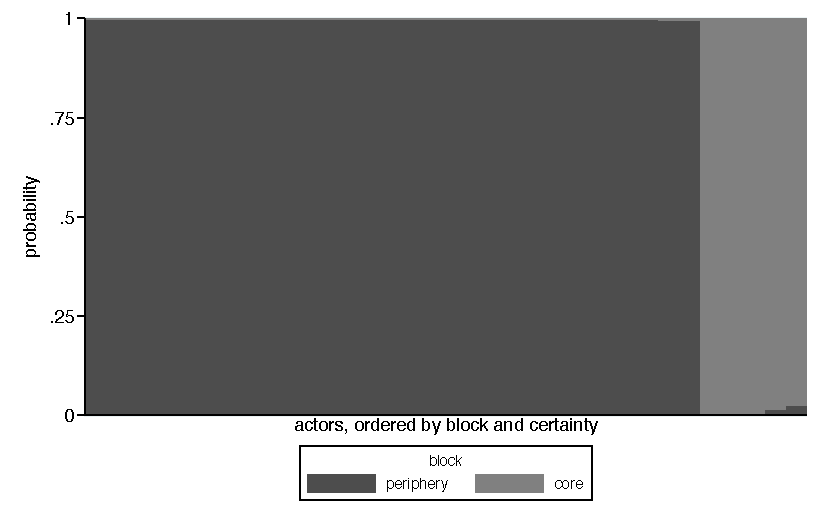
\includegraphics[width=0.7\textwidth]{fig/fig_member.pdf}
\caption{\texttt{nwsbmplot, type(membership) blocklabels(periphery core) colors(gray) title("")} after the two-block fit of the karate club.}\label{fig:member}
\end{figure}

\paragraph{Block graph.} \opt{type(blocks)} draws the blocks as nodes, the size proportional to the number of actors, and the connectivity between blocks as lines whose width follows the entries of \texttt{e(pi)} relative to the largest entry; entries below 2 percent of it are not drawn. One-mode blocks sit on a circle; for a directed network the two directions of a pair of blocks are drawn as two arrows side by side; the blocks of a two-mode network sit in two columns. Connectivity within a block is not drawn. Figure~\ref{fig:blocks} shows the three-block fit of the karate club: block 2 (five members) is the hub between the two large blocks, which are hardly tied to each other.
\begin{figure}[htbp]\centering
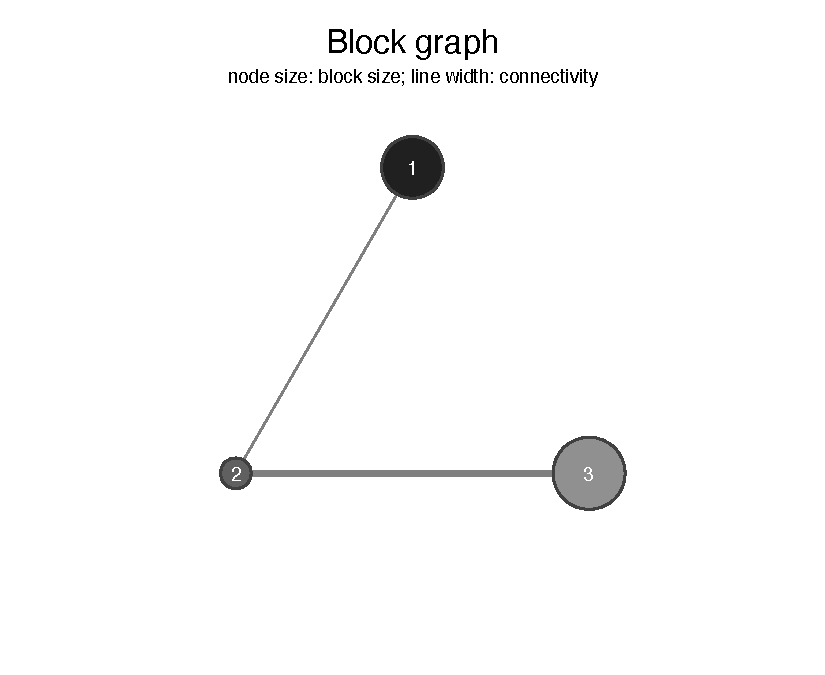
\includegraphics[width=0.62\textwidth]{fig/fig_blocks.pdf}
\caption{\texttt{nwsbmplot, type(blocks) colors(gray)} after \texttt{blocks(3)} on the karate club.}\label{fig:blocks}
\end{figure}

\paragraph{Two-mode matrix.} For a two-mode network the rows of the matrix plot are the actors of mode~1 and the columns those of mode~2, each ordered by its blocks (Figure~\ref{fig:davis}).
\begin{figure}[htbp]\centering
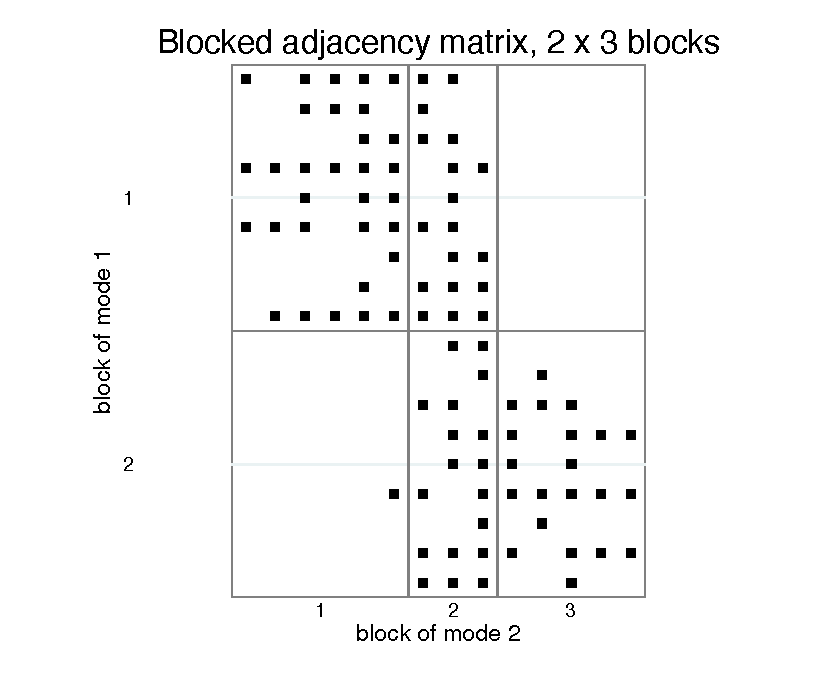
\includegraphics[width=0.62\textwidth]{fig/fig_davis.pdf}
\caption{\texttt{nwsbmplot, type(matrix)} after the two-mode fit of the Southern women: women in the rows, events in the columns.}\label{fig:davis}
\end{figure}

\section{Saving and exporting}
\opt{name()} keeps the graph in memory, \opt{saving()} writes a \texttt{.gph} file, and \opt{export()} writes a file whose format follows the extension. The figures of this chapter were made with commands of the form
\begin{lstlisting}
nwsbmplot, type(matrix) shade blocklabels(periphery core) export(fig_matrix.pdf) xsize(5.5) ysize(5.5)
\end{lstlisting}
\texttt{xsize()} and \texttt{ysize()} are options of \texttt{twoway} and set the size of the exported graph in inches.
